% !TeX spellcheck = en_US
% !TeX root = ../Tom_Sandmann-master_thesis
\chapter{\texorpdfstring{Attacking \fourq}{Attacking FourQ}} \label{chp: Attacking FourQ}
\lettrine[lhang = 0.4, findent=-30pt, lines=4]{\textbf{
		\initfamily \fontsize{20mm}{20mm} \selectfont I
		\normalfont}}{n} 
this chapter, we describe how we attack {\fourq}.
In \Cref{chp: Side Channel Attacks}, we have seen how we can apply an \emph{Online Template Attack} (OTA) to a very simple left-to-right double-and-add always algorithm that performed its calculations in constant time.
When applying an OTA to {\fourq}, we have to slightly change our approach to attack the key bits compared to the example we gave in \Cref{chp: Side Channel Attacks}.
In addition, the attack itself is also more difficult, as it (at first sight) requires us to inverse both the scalar recoding and scalar decomposition routines when generating the templates used in attacking the scalar.
We discuss these practicalities in this chapter.

% !TeX spellcheck = en_US
% !TeX root = ../Tom_Sandmann-master_thesis
\section{\texorpdfstring{Applying online template attacks to \fourq}{Applying online template attacks to FourQ}}
In \Cref{algo: FourQ's scalar multiplication} in \Cref{chp: FourQ}, we can see the complete scalar multiplication of \fourq.
In order to retrieve the secret scalar, we need to obtain the $s_i$ and $d_i$ values that are applied in each iteration.
Recall that in the case of an OTA, the attacker can only capture one \emph{target trace} of the device under attack (i.e. the \emph{target device}).
In addition, we assume that the attacker knows the input point that belongs to this trace.
On the attacker's device, the attacker has full control over the implementation (which is the same implementation responsible for the captured \emph{target trace}).
This means that the attacker can change the scalar, but also the base point in the scalar multiplication.
We now describe how we apply an OTA to {\fourq}.
%
\begin{itemize}
	\item \textbf{Attacking the first digit-column}. 
	If we take a look at the actual scalar multiplication algorithm in \Cref{algo: FourQ's scalar multiplication}, we can see that $s_{64}$ determines the sign of the first element taken from the lookup table $T$.
	Which element is taken from this table is determined by the value $d_{64}$, which is unknown to us in the captured \emph{target trace}.
	After the initial assignment in \Cref{lst:fourq scalar mult:initial assignment}, the doubling operation of this initial value (i.e. loop at iteration $i = 63$) is done at \Cref{lst:fourq scalar mult:double oper}.
	This is the first doubling operation we are going to attack.
	If we take a look at the general scalar recoding algorithm employed by {\fourq} in \Cref{algo: Protected Recoding Algorithm for the GLV-SAC Representation} (in \Cref{chp: FourQ})%
	\footnote{In the case of \fourq, we have $l = 65$ and $m = 4$.}
	%
	, we can see that $b_{64}$ is always assigned a value of one, and that this value is used in the main loop as $s_{64}$.
	As we already know that the value of $s_{64} = 1$, we are left to guess the value of $d_{64}$, which is a 3-bit value.
	Our goal in the first `iteration' of our OTA is to try all of the possible $d_{64}$ values (i.e. our templates), such that we can obtain the corresponding power traces of the doubling operations.
	We then use these templates to find the one that matches best with the corresponding part of the \emph{target trace} (i.e. the first doubling operation).
	
	\item \textbf{Attacking the remaining digit-columns}. Once we have found the template (and its corresponding $d_{64}$ value) that matched the best with our \emph{target trace} at the first doubling operation, its time to attack the remaining digit-columns.
	At \Cref{lst:fourq scalar mult:add oper}, we see that both $s_i$ and $d_i$ determine the new value of the variable $Q$. 
	In the next iteration $i - 1$, this variable $Q$ is doubled again. To find out which values of $s_i$ and $d_i$ were used, we have to generate all of the possible templates for these values. This are at most 16 possible templates (3 bits for $d_i$ and 1 bit for $s_i$).
	Note that we need to compare each of the corresponding template traces at the $(i - 1)^\mathrm{th}$ doubling operation to attack the $d_i$ and $s_i$ values used in the addition operation in the $i^\mathrm{th}$ iteration.
	We are then iteratively constructing the matrix that corresponds to the recoded scalars of {\fourq}.
	Using these scalar values, we need to invert the scalar decomposition applied to the secret scalar to obtain the `original scalar' of the scalar multiplication that corresponds to the \emph{target trace}.  
	
	\item \textbf{Attacking the last digit-column}. We cannot use a doubling operation to attack the last digit-column and sign ($s_{0}$ and $d_0$) in the $0^\mathrm{th}$ iteration, as the main loop ends after this iteration. 
	There are however two other ways to attack the last digit-column and its corresponding sign. 
	One way is to use the generated templates for the addition operation involving $d_0$ and $s_0$, and use this operation instead to match the template traces with the target trace.
	Another way would be to brute force these last values, and see which output of the scalar multiplication gives the correct results.
\end{itemize}
%
As mentioned in \cite{batina2014online}, we can also use the addition operation in the $i^\mathrm{th}$ iteration together with the doubling operation in the $(i - 1)^\mathrm{th}$ iteration to attack digit-column $(s_i, d_i)$.
In this way, we can increase the chance of choosing the correct template.
This is however only possible when attacking the digit-columns not used in the first or last iteration (i.e digit-columns $(s_{63}, d_{63})$ up to $(s_{1}, d_{1})$).
% !TeX spellcheck = en_US
% !TeX root = ../Tom_Sandmann-master_thesis
\section{An attempt to inverse the scalar recoding} \label{sec: An attempt to inverse the scalar recoding}
To obtain templates for the OTA, we need to find recoded scalars with specific values at the digit-columns in the corresponding recoded matrix.
As we can change the value of the scalar used in {\fourqs} scalar multiplication, we need to obtain a scalar that, once decomposed and recoded, has the expected digit-column values in it.
To determine which decomposed multiscalar belongs to our wanted recoded matrix, we have to inverse the scalar recoding for this matrix.
We first take a look at the operations in the scalar recoding algorithm shown in \Cref{algo: Protected Recoding Algorithm for the GLV-SAC Representation}.
We can see that in \Cref{lst:scalar recoding general:scalar update}, the value of the scalar gets updated in each iteration by taking the floor of its current value divided by 2 (i.e. a bit shift of 1 to the right) and subtracting the floor of $b_i^j$ divided by 2.
In \Cref{lst:scalar recoding general:digit column value}, we see that the value $b_i^j$ is assigned a value that is the result of taking bit $i$ of the sign-aligner and multiplying it with the very first bit of scalar $k_j$.
So what are the possible values for these variables?
%
\begin{itemize}
	\item $\bm{b_i^j = b_i^J \cdot k_0^j}$. We know that, once the sign-aligner is converted to signed non-zero form (\Cref{lst:scalar recoding general:signed-nonzero start,lst:scalar recoding general:signed-nonzero oper,lst:scalar recoding general:signed-nonzero end})% <--- no space after the comma
	, all of its values at position $i$ will be either $1$ or $-1$: $b_i^J \in \{1, -1\}$. As the value $k_i^j \in \{0, 1\}$ (as all of the scalars are binary numbers in signed form), we have $b_i^j \in \{0, 1, -1\}$.
	
	\item $\bm{k_j = \lfloor k_j / 2\rfloor - \lfloor b_i^j / 2 \rfloor}$. We know that $b_i^j \in \{0, 1, -1\}$. Therefore, we have $\lfloor b_i^j / 2 \rfloor \in \{0, -1\}$. Note that the $-1$ is due to the fact that $\lfloor -1 / 2 \rfloor = -1$.
\end{itemize}
%
As the floor operation applied to the scalar $k_j$ divided by 2 is in essence a bit shift, we can see that this bitshift is done $65$ times (i.e for $j \in [0, 64]$).
As we are working with $64$-bit integers, one would expect that the value of the scalar becomes zero after 64 bitshifts. However, the subtraction of $\lfloor  b_i^j / 2 \rfloor$ from the shifted scalar can also result in an addition of 1.
Therefore, only after $65$ bitshifts the value of $k_j$ will be zero.
We know that all $k_j$'s will have a value of zero once the recoding algorithm has been applied.
Lets see what happens if we try to obtain the original multiscalar by applying the algorithm in reversed order.
As we know, a bitshift is not a completely irreversible operation.
In the case of a right bitshift, we loose the first bit of the scalar (i.e. the bit indicating the parity of the scalar).
Due to the bitshift and subtraction occurring at \Cref{lst:scalar recoding general:scalar update} of the algorithm, we somehow have to guess what the value in the previous iteration would have been.
So what are these possible values.
This depends on the parity of the scalar used.
Assume we have the result $r = (((d >> 1) << 1) + c)$ with $c \in \{0, 1\}$ and $d \in \mathbb{N}$.
By finding all possible outcomes for $r$ and $c$ with $d$ being either odd or even, we know how many possibilities there are when inverting the operation of \Cref{lst:scalar recoding general:scalar update} in the recoding algorithm. 
The results can be seen in \Cref{tbl: inversion of floor function}.
%
\begin{table}
	\centering
	%	
	\begin{tabular}{*3c}
		\toprule
		& $\bm{d \in \mathbb{N}}$ & $\bm{d \in 2\mathbb{N} \setminus \{0\} }$ \\
		\midrule
		$\bm{c = 0}$ & $0$ & $1$ \\
		$\bm{c = 1}$ & $-1$ & $0$ \\
		\bottomrule
	\end{tabular}
	%
	\captionof{table}{Possible outcomes of the equation $r = (((d >> 1) << 1) + c)$ with $c \in \{0, 1\}$ and $d \in \mathbb{N}$ being either odd or even. This table shows the possible values of $k_j$ if we would try to find its original value after we already applied the operation at \Cref{lst:scalar recoding general:scalar update} of \Cref{algo: Protected Recoding Algorithm for the GLV-SAC Representation}.}
	\label{tbl: inversion of floor function}
\end{table}
%
We can see that $r \in \{0, 1, -1\}$, which gives us an idea of the number of possibilities when trying to undo the operation at \Cref{lst:scalar recoding general:scalar update} of the recoding algorithm once it has been applied.
In each iteration of the algorithm, it seems like we need to guess three possibilities to obtain the correct value for iteration $i - 1$: $k_j << 1$, $(k_j << 1) - 1$ and $(k_j << 1) + 1$. 
This seems to be impossible, as this would require us to try $3^{64}$ values.
However, at every moment in time, we only need to make sure that the digit-column for which we are trying to generate templates has a specific value (and all the previous digit-columns we already attacked).
It therefore seems to be the case that the values of the other digit-columns do not matter.
To see if we can make this work, we take a look at the example shown in \cite[Example 1]{faz2015efficient}.
In this example, they also have a multiscalar consisting of four scalars ($m = 4$) having a length of $l = 5$. 
The decomposition of the `original scalar' is given as $kP = 11P_0 + 6P_1 + 14P_2 + 3P_3$. 
If we arrange the scalars in matrix form and apply the recoding, we get the following:
%
\begin{equation*}
%
\begin{bmatrix}
k_0 \\
k_1 \\
k_2 \\
k_3 
\end{bmatrix}
%
\equiv
%
\begin{bmatrix}
0 & 1 & 0 & 1 & 1 \\
0 & 0 & 1 & 1 & 0 \\
0 & 1 & 1 & 1 & 0 \\
0 & 0 & 0 & 1 & 1 
\end{bmatrix}
%
\equiv
%
\begin{bmatrix}
1 & \bar{1} & 1 & \bar{1} & 1 \\
1 & \bar{1} & 0 & \bar{1} & 0 \\
1 & 0 & 0 & \bar{1} & 0 \\
0 & 0 & 1 & \bar{1} & 1
\end{bmatrix}
%
\end{equation*}
%
We are going to attack the leftmost digit-column (just like the one that would be used in the very first iteration of {\fourqs} scalar multiplication algorithm).
In this case, this is digit-column $d_4$.
Our first step would be to find a multiscalar that produces the output in the matrix that we want to have for $d_4$.
We assume that this is the exact same template as the one produced by the `secret' scalar: $\mathbb{K}_4 = \left[ 011 \right]$ or $d_4 = 3$.
Now we try to find the remaining entries in the recoding matrix. 
For simplicity, we show our attempt by only taking the first scalar into account (i.e. $k_1$). 
Recall the operation that updates the scalar in each iteration:
%
\begin{equation*}
k_j = \lfloor k'_j / 2 \rfloor - \lfloor b_i^j \rfloor \equiv \lfloor k'_j / 2 \rfloor - \lfloor (b_i^J \cdot k_0^{\prime j} ) / 2 \rfloor 
\end{equation*}
%
with $k_j'$ denoting the value of $k_j$ in the current iteration before it was updated (i.e the value of $k_j$ after the previous iteration $i - 1$ finished).
The attempt is shown below.
%
\begin{itemize}
	\item \textbf{Iteration} $\bm{i = 4}$. 	We know that $k_1 = \lfloor k'_1 / 2 \rfloor - \lfloor (b_4^J \cdot k_0^{\prime 1} ) / 2 \rfloor = 0$ with $k'_1 \in \{0, 1\}$ (note that $-1$ is not possible as the intermediate values of the scalar remain positive throughout the entire algorithm). 
	In addition, we also know that $b_4^J = 1$.
	This gives us two possibilities:
	%
	\begin{itemize}
		\item $\bm{ \lfloor k'_1 / 2 \rfloor = 0 }$ \textbf{and} $ \bm{ \lfloor (b_3^J \cdot k_0^{\prime 1}) / 2 \rfloor = 0 }$. 
		$\lfloor k'_1 / 2 \rfloor = 0$ can only happen if $k'_1 \in \{0, 1\}$. $\lfloor (b_3^J \cdot k_0^{\prime 1}) / 2 \rfloor = 0$ can only happen if $b_3^J \cdot k_0^{\prime 1} \in \{0, 1\}$. This implies that $b_4^J = 1$ and $ k_0^{\prime 1} = 1$. The latter is only possible if $k'_1 = 1$.
		
		\item  $\bm{ \lfloor k'_1 / 2 \rfloor = 1 }$ \textbf{and} $ \bm{ \lfloor (b_3^J \cdot k_0^{\prime 1}) / 2 \rfloor = 1 }$. 
		$ \lfloor k'_1 / 2 \rfloor = 1$ is only possible if $k'_1 \in \{0, 1\}$. However, this contradicts with the fact that $k'_1 \in \{0, 1\}$ \Lightning.
	\end{itemize}
	%
	
	\item \textbf{Iteration} $\bm{i = 3}$. We know that $k_1 = \lfloor k'_1 / 2 \rfloor - \lfloor (b_3^J \cdot k_0^{\prime 1}) / 2 \rfloor = 1$ with $k'_1 \in \{1, 2, 3\}$. This gives us two possibilities:
	%
	\begin{itemize}
		\item $\bm{ \lfloor k'_1 / 2 \rfloor = 0 }$ \textbf{and} $ \bm{ \lfloor (b_3^J \cdot k_0^{\prime 1}) / 2 \rfloor = -1 }$. 
		$\lfloor k'_1 / 2 \rfloor = 0 $ can only happen if $k'_1 = 1$. $\lfloor (b_3^J \cdot k_0^{\prime 1}) / 2 \rfloor = -1$ can only happen if $b_3^J \cdot k_0^{\prime 1} \in \{-2, -1 \}$. This means that $k_0^{\prime 1} = 1$ and $b_3^J = -1$.
		
		\item $\bm { \lfloor k'_1 / 2 \rfloor = 1 }$ \textbf{and} $ \bm{ \lfloor (b_3^J \cdot k_0^{\prime 1}) / 2 \rfloor = 0 }$.
		$\lfloor k'_1 / 2 \rfloor = 1$ can only happen if $k'_1 \in \{2, 3\}$. $ \lfloor (b_3^J \cdot k_0^{\prime 1}) / 2 \rfloor = 0$ can only happen if $b_3^J \cdot k_0^{\prime 1} \in \{0, 1\}$. This gives the following combinations of values:
		%
		\begin{itemize}
			\item $b_3^J = -1$ and $ k_0^{\prime 1} = 0$ (implies $k'_1 = 2$)
			\item $b_3^J = 1$ and $ k_0^{\prime 1} = 0$ (implies $k'_1 = 2$)
			\item $b_3^J = 1$ and $ k_0^{\prime 1} = 1$ (implies $k'_1 = 3$)
		\end{itemize}
		%
		For the sake of simplicity, we assume to guess $k'_1 = 1$ which gives $k_0^{\prime 1} = 1$.
	\end{itemize}
	%
	\item \textbf{Iteration} $\bm{i = 2}$. We know that $k_1 = \lfloor k'_1 / 2 \rfloor - \lfloor (b_2^J \cdot k_0^{\prime 1}) / 2 \rfloor = 1$ with $k'_1 \in \{1, 2, 3\}$. This gives us two possibilities:
	%
	\begin{itemize}
		\item $\bm{ \lfloor k'_1 / 2 \rfloor = 0 }$ \textbf{and} $ \bm{ \lfloor (b_2^J \cdot k_0^{\prime 1}) / 2 \rfloor = -1 }$. 
		$\lfloor k'_1 / 2 \rfloor = 0 $ can only happen if $k'_1 = 1$. $\lfloor (b_2^J \cdot k_0^{\prime 1}) / 2 \rfloor = -1$ can only happen if $b_2^J \cdot k_0^{\prime 1} \in \{-2, -1\}$. This means that $k_0^{\prime 1} = 1$ and $b_2^J = -1$.
		
		\item $\bm { \lfloor k'_1 / 2 \rfloor = 1 }$ \textbf{and} $ \bm{ \lfloor (b_2^J \cdot k_0^{\prime 1}) / 2 \rfloor = 0 }$.
		$\lfloor k'_1 / 2 \rfloor = 1$ can only happen if $k'_1 \in \{2, 3\}$. $ \lfloor (b_2^J \cdot k_0^{\prime 1}) / 2 \rfloor = 0$ can only happen if $b_2^J \cdot k_0^{\prime 1} \in \{0, 1\}$. 
		This gives the following combinations of values:
		%
		\begin{itemize}
			\item $b_2^J = -1$ and $ k_0^{\prime 1} = 0$ (implies $k'_1 = 2$)
			\item $b_2^J = 1$ and $ k_0^{\prime 1} = 0$ (implies $k'_1 = 2$)
			\item $b_2^J = 1$ and $ k_0^{\prime 1} = 1$ (implies $k'_1 = 3$)
		\end{itemize}
		%
		For the sake of simplicity, we assume to guess $k'_1 = 2$ which gives $k_0^{\prime 1} = 0$.
	\end{itemize}
	%
	\item \textbf{Iteration} $\bm{i = 1}$. We know that $k_1 = \lfloor k'_1 / 2 \rfloor - \lfloor (b_1^J \cdot k_0^{\prime 1}) / 2 \rfloor = 2$ with $k'_1 \in \{3, 4, 5\}$. This gives us two possibilities:
	%
	\begin{itemize}
		\item $\bm{ \lfloor k'_1 / 2 \rfloor = 1 }$ \textbf{and} $ \bm{ \lfloor (b_1^J \cdot k_0^{\prime 1}) / 2 \rfloor = -1 }$. 
		$\lfloor k'_1 / 2 \rfloor = 1 $ can only happen if $k'_1 \in \{2, 3\}$ (i.e. $k'_1 = 3$). $\lfloor (b_1^J \cdot k_0^{\prime 1}) / 2 \rfloor = -1$ can only happen if $b_1^J \cdot k_0^{\prime 1} \in \{-2, -1\}$. This means that $k_0^{\prime 1} = 1$ and $b_1^J = -1$.
		
		\item $\bm { \lfloor k'_1 / 2 \rfloor = 2 }$ \textbf{and} $ \bm{ \lfloor (b_1^J \cdot k_0^{\prime 1}) / 2 \rfloor = 0 }$.
		$\lfloor k'_1 / 2 \rfloor = 2$ can only happen if $k'_1 \in \{4, 5\}$. $ \lfloor (b_1^J \cdot k_0^{\prime 1}) / 2 \rfloor = 0$ can only happen if $b_1^J \cdot k_0^{\prime 1} \in \{0, 1\}$. 
		This gives the following combinations of values:
		%
		\begin{itemize}
			\item $b_1^J = -1$ and $ k_0^{\prime 1} = 0$ (implies $k'_1 = 4$)
			\item $b_1^J = 1$ and $ k_0^{\prime 1} = 0$ (implies $k'_1 = 4$)
			\item $b_1^J = 1$ and $ k_0^{\prime 1} = 1$ (implies $k'_1 = 5$)
		\end{itemize}
		%
		For the sake of simplicity, we assume to guess $k'_1 = 3$ which gives $k_0^{\prime 1} = 1$.
	\end{itemize}
	%
	\item \textbf{Iteration} $\bm{i = 0}$. We know that $k_1 = \lfloor k'_1 / 2 \rfloor - \lfloor (b_0^J \cdot k_0^{\prime 1}) / 2 \rfloor = 3$ with $k'_1 \in \{5, 6, 7\}$. This gives us two possibilities:
	%
	\begin{itemize}
		\item $\bm{ \lfloor k'_1 / 2 \rfloor = 2 }$ \textbf{and} $ \bm{ \lfloor (b_0^J \cdot k_0^{\prime 1}) / 2 \rfloor = -1 }$. 
		$\lfloor k'_1 / 2 \rfloor = 2 $ can only happen if $k'_1 \in \{4, 5\}$ (i.e. $k'_1 = 5$). $\lfloor (b_0^J \cdot k_0^{\prime 1}) / 2 \rfloor = -1$ can only happen if $b_0^J \cdot k_0^{\prime 1} \in \{-2, -1\}$. This means that $k_0^{\prime 1} = 1$ and $b_1^J = -1$.
		
		\item $\bm { \lfloor k'_1 / 2 \rfloor = 3 }$ \textbf{and} $ \bm{ \lfloor (b_0^J \cdot k_0^{\prime 1}) / 2 \rfloor = 0 }$.
		$\lfloor k'_1 / 2 \rfloor = 3$ can only happen if $k'_1 \in \{6, 7\}$. $\lfloor (b_0^J \cdot k_0^{\prime 1}) / 2 \rfloor = 0$ can only happen if $b_1^J \cdot k_0^{\prime 1} \in \{0, 1\}$. 
		This gives the following combinations of values:
		%
		\begin{itemize}
			\item $b_0^J = -1$ and $ k_0^{\prime 1} = 0$ (implies $k'_1 = 6$)
			\item $b_0^J = 1$ and $ k_0^{\prime 1} = 0$ (implies $k'_1 = 6$)
			\item $b_0^J = 1$ and $ k_0^{\prime 1} = 1$ (implies $k'_1 = 7$)
		\end{itemize}
		%
		For the sake of simplicity, we assume to guess $k'_1 = 6$ which gives $k_0^{\prime 1} = 1$.
	\end{itemize}
	%
\end{itemize}
%
As you can see, we have three possibilities for obtaining a specific value for the last bit in digit-column $\mathbb{K}_4$.
For the other most-significant bits in the remaining digit-columns, we have four combinations to guess. This gives a total number of $3 \cdot 4^4 = 768$ combinations for this very simple example. In the case of {\fourq} where we have $l = 65$, this would give us $3 \cdot 4^{64}$ possible combinations (a 130-bit value), which is clearly unfeasible to brute force. 
%
\begin{table}[H]
	\centering
	\begin{tabular}{*6c}
		\toprule 
		& \multicolumn{5}{c}{iteration $i$} \\
		\cline{2-6}
		& \textbf{0} & \textbf{1} & \textbf{2} & \textbf{3} & \textbf{4} \\
		\midrule
		$b_i^J$ & 1 & -1 & 1 & -1 & 1 \\
		$k_0^j$ & 0 & 1 & 0 & 1 & 1 \\
		$b_i^j$ & 0 & -1 & 0 & -1 & 1 \\
		$k_j$ & 3 & 2 & 1 & 1 & 0  \\
		\bottomrule
	\end{tabular}
	\captionof{table}{intermediate values for the scalar recoding iteration with $j = 1$ and $k_1 = 6$.}
\end{table}
%
\begin{figure}[H]
	\centering
	\subfloat[Outcome ranges for the function $\lfloor \frac{x \cdot y}{2}\rfloor$ with $x \in \{1, -1\}$ and $y \in \{0, 1\}$ but $y$'s exact value being unknown.]{
	%
	\centering
	\begin{tabular}{*2c}
		\toprule
		& $\lfloor \frac{x \cdot y}{2}\rfloor$ \\
		\midrule
		$x = 1$ & $y$ \\
		$x = -1$ & $-y$ \\
		\bottomrule
	\end{tabular}
	%
	}
	%	
	\hspace{1cm}
	%		
	\subfloat[Outcome ranges for the function $\lfloor \frac{x \cdot y}{2}\rfloor$ with $y \in \{0, 1\}$ and $x \in \{-1, 1\}$ but $x$'s exact value being unknown.]{
	%
	\centering
	\begin{tabular}{*2c}
		\toprule
		& $\lfloor \frac{x \cdot y}{2}\rfloor$ \\
		\midrule
		$y = 0$ & $0$ \\
		$y = 1$ & $x$ \\
		\bottomrule
	\end{tabular}
	%
	}
	\captionof{figure}{Possible outcomes for the function $\lfloor \frac{x \cdot y}{2}\rfloor$ with either $x$ or $y$ being unknown.}
\end{figure}
%
Fortunately, we can circumvent the inversion of the recoding by changing the hardware implementation in such a way that it takes a decomposed scalar instead of a scalar that still needs to be decomposed. 
The implementation still remains the same, but instead of assigning the results of the decomposition to the corresponding multiscalar, we take the values of the decomposed scalar directly and assign them to their corresponding signals.
It would however still be interesting to see if it is possible to invert the scalar recoding in such a way that you can create a recoded multiscalar.
If we convert this multiscalar back to the original scalar and apply decomposition and recoding, it should still have the wanted values at the specific digit-columns in the recoded matrix.
This would make a template attack against hardware implementations of {\fourq} possible in an even more restricted setting where the attacker does have a similar device, but where its implementation cannot be changed. 
This could however be a whole research project on its own, and is left as an open problem for others.
% !TeX spellcheck = en_US
% !TeX root = ../Tom_Sandmann-master_thesis
\section{Determining the offsets} \label{sec: Determining the offsets}
Given the power trace of both the target trace and the template trace, we need to extract the relevant doubling and/or addition operations from these traces and correlate them.
This requires us to determine the offsets into these trace that indicate where the required operation starts and how long it lasts.
To determine these offsets, we add a trigger to our hardware design that is high between the start and end of these operations.
Determining these exact values was done adding by adding output statements to the \emph{control FMS} (see \Cref{chp: FourQ On Hardware}).
This component knows exactly when the scalar multiplication is executing within the main loop.
Unfortunately, there is only \emph{one} state which indicates that either the doubling or addition operation is performed, but not exactly when it starts or ends.
From \cite{jarvinen2016four}, we know that an iteration of the main loop of {\fourq} starts when the value of the program counter equals 4215 and ends when this value is 4568.
We also know that the main loop starts with the doubling operation.
Thus, it remains unclear when (1) a doubling operations ends and when (2) an addition operation starts.
To obtain these unknown offsets (and also to verify the known ones), we make use of a reference implementation of {\fourq} available on GitHub%
\footnote{\url{https://bifurcation.github.io/fourq/}} that belongs to an Internet-Draft of {\fourq} \cite{ladd-cfrg-4q-01}.
This implementation is dubbed \texttt{Curve4Q} and follows the approach described in the original paper.
It therefore does \emph{not} make use of the newly introduced representation $\bm{R_5}$ used in the proposed hardware design of {\fourq} \cite{jarvinen2016four}.
Thus, we add the conversion functions as shown in \Cref{appendix: curve4q modifications} to this reference implementation.
We then change the code in such a way that these newly introduced conversion functions are used in the table generation phase and in the initial assignment to $Q$.
In addition, we also add print statement to the start and end of the actual \texttt{DBL} and \texttt{ADD} methods.
By also printing the output of the Field Arithmetic Unit (FAU)%
\footnote{This is done by making use of the \mintinline{text}{image_pb.vhd} VHDL package written by Ben Cohen, which can be found \href{http://web.archive.org/web/20070202003755/http://members.aol.com/vhdlcohen/vhdl/Models.html}{online}.
A more recent version of such a package is the \mintinline{text}{txt_util.vhd} VHDL package, written by Øyvind Harboe.}
%
and the program counter, we can use the output of both the reference implementation and the FAU to determine at which program counter values the \texttt{DBl} and \texttt{ADD} operations start and end.
The results can be seen in \Cref{tbl: FourQ DBL/ADD start/end values}.
%
\begin{table}
	\centering
	%
	\begin{tabular}{*3c}
		\toprule
		& \textbf{start} & \textbf{end} \\
		\midrule
		\texttt{DBL} & 4216/4217 & 4380/4381 \\
		\texttt{ADD} & 4373/4374 & 4564/4565 \\
		\bottomrule
	\end{tabular}
	%
	\captionof{table}{Values of the program counter in the hardware design of {\fourq} at which the \texttt{DBL} and \texttt{ADD} operations start and end. The value of the program counter points to instructions in program ROM that are used to control the operations needed to compute the scalar multiplications of {\fourq.} }
	\label{tbl: FourQ DBL/ADD start/end values}
\end{table}
%
We used these program counter values to add a trigger in the given hardware design that has a high signal on the start and end of each operation.
As the main loop of {\fourq} consists of 64 points additions \emph{and} 64 doubling operations, this gives us 128 rising and falling edges in the corresponding power trace of this trigger.

As described in \cite{batina2014online}, we can also focus on a single operation within this doubling operation. 
Focusing on the first squaring operation in doubling formulas described in \cite{ladd-cfrg-4q-01} gives us different values for the program counter. These values can be seen in \Cref{tbl: FourQ DBL/ADD start/end values first squaring}.
%
\begin{table}
	\centering
	%
	\begin{tabular}{*3c}
		\toprule
		& \textbf{start} & \textbf{end} \\
		\midrule
		\texttt{DBL} & 4216/4217 & 4251 \\
		\texttt{ADD} & 4373/4374 & 4489 \\
		\bottomrule
	\end{tabular}
	%
	\captionof{table}{Values of the program counter in the hardware design of {\fourq} at which the \texttt{DBL} and \texttt{ADD} operations start and end. In this case, instead of taking the whole doubling operation into account, only the first squaring in the doubling and addition operation is used to find the corresponding program counter values.}
	\label{tbl: FourQ DBL/ADD start/end values first squaring}
\end{table}
%
The corresponding power trace when using the start/end values for the \emph{addition} operation as mentioned in \Cref{tbl: FourQ DBL/ADD start/end values}, and for the \emph{doubling} operation as mentioned in \Cref{tbl: FourQ DBL/ADD start/end values first squaring}, can be seen in \Cref{fig: oper_trigger_trace}.
%
\begin{figure}
	\centering
	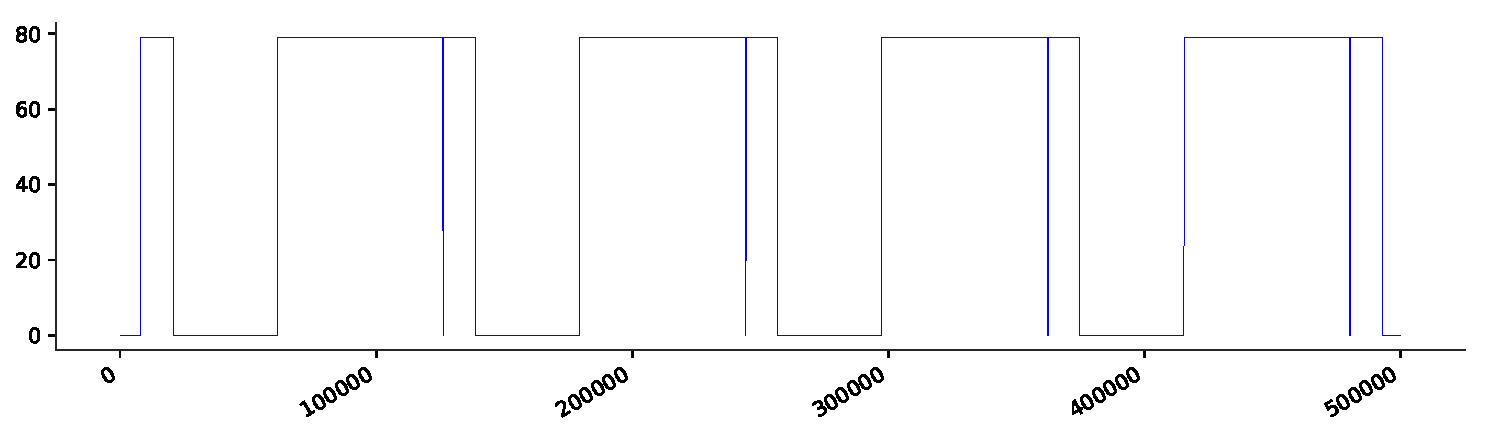
\includegraphics[scale=0.6]{traces/oper_trigger_trace}
	\captionof{figure}{Power trace that indicates at which samples the doubling and addition operations start and end. Instead of taking the whole doubling operation into account, we only determine where the very first squaring happens. This explains why the doubling operation consist of less samples than the addition operation. }
	\label{fig: oper_trigger_trace}
\end{figure}
%
Given this power trace, we need to determine the indices at which a rising edge starts and how long it stays high (i.e. determine the relative index of the start of the corresponding falling edge).
Initially, our approach was to calculate the difference between consecutive elements in this trigger trace without any preprocessing. 
If the difference of two successive elements is high, it indicates that we are approaching a rising/falling edge (depending on the sign of this difference).
The success of this approach however depends on the sampling rate used.
If a low sampling rate is used, the difference between two successive elements can be higher.
In the case of a higher sampling rate, this difference will be much smaller.
Therefore, it is hard to choose a correct threshold to determine the indices of the rising and falling edges in this trigger trace.
To solve this, we decided to preprocess the trace by rounding all values below a threshold to zero.
One has to make sure that this threshold is lower than the values between a rising and falling edge.
Applying the method we described first now correctly yields the offsets at which operations start and end.

The previously described method still depends on the vertical offset of the operation trigger trace. 
A method that works regardless the vertical offset is shown in \Cref{algo: determining offsets}.
In the end, we decided to stick with this generic method.
The algorithm works by first determining the average of the minimum and maximum value in the trigger trace.
We then determine the greatest lower bound (GLB) and least upper bound (LUB) for all values smaller and bigger than this average respectively.
Our threshold $\mu$ now becomes the average of GLB and LUB.
All values in the trigger trace that are bigger or equal to this threshold are clipped to the maximum value, while values smaller are clipped to the minimum value. 
We then calculate the consecutive differences of all the samples in this trigger trace.
We can now determine the rising and falling edge indices by checking whether these absolute differences are bigger than our threshold $\mu$.
The offsets can now easily be found by taking the difference between these indices.
Given a pair of successive edge indices, only those indices are taken into account for which the first edge index corresponds to a rising edge (i.e. has a positive difference or its value is bigger than $\mu$).
%
\begin{algorithm}
	\algorithmicrequire A power trace $T$ of the trigger that indicates when one or more doubling/addition operations start/end. \\
	\algorithmicensure The offsets and durations to these operations.
	%	
	\begin{algorithmic}[1]
		\State $\text{min\_max\_avg} = (\max(T) + \min(T)) / 2$
		\State $T_H = \{s \mid s \in T, s \ge \text{min\_max\_avg} \}$
		\State $T_L = \{s \mid s \in T, s < \text{min\_max\_avg} \}$
		\State $\text{lub} = \sup(T_H)$ \Comment{Least Upper Bound (LUB)}
		\State $\text{glb} = \inf(T_L)$ \Comment{Greatest Lower Bound (GLB)}
		\State $\mu = (\text{glb} + \text{lub}) / 2$
		\State For all $s$ in $T$: if $s \ge \mu$ clip value to $\max(T)$, else clip value to $\min(T)$
		\State $\texttt{succ\_diffs}= \{T[n + 1] - T[n] \mid n \in [1, \#T) \}$ \Comment{Calculate the first order difference}
		\State $\texttt{edges} = \{\operatorname{idx}(d) + 1, d\in D \mid \abs{d} \ge \mu \}$ \Comment{Determine offsets}
		\State $\texttt{offsets} = \{(\texttt{edges}[n], \texttt{edges}[n + 1] - \texttt{edges}[n]) \mid n \in [0, \#\texttt{edges} ], \texttt{offsets}[n] > \mu \}$
		\State \textbf{Return} $\texttt{offsets}$
	\end{algorithmic}
	%
	\captionof{algorithm}{Given a power trace that contains the signals of the operations to attack, determine the offsets to these operations.}
	\label{algo: determining offsets}
\end{algorithm}
%
% !TeX spellcheck = en_US
% !TeX root = ../Tom_Sandmann-master_thesis
\section{Matching the templates} \label{sec: Matching the templates}
Using the method as described in \Cref{algo: determining offsets} of \Cref{sec: Determining the offsets} to determine the offsets, we applied the OTA to the {\fourq} hardware design using the SAKURA-G board.
For the very first iteration, the target trace of the relevant doubling operation together with the corresponding template traces can be seen in \Cref{fig: OTA first iteration target example} and \Cref{fig: OTA first iteration templates example} respectively.
An overlap of the template traces can be seen in \Cref{fig: OTA first iteration template traces overlap}.
All of these traces are captured with a sampling rate of 1GSa/s without any bandwidth or noise filter applied.
The signal coupling of the channels was set to $\mathrm{DC}50\ohm$.
The operation speed of the {\fourq} design was set to 1.5MHz (which is the default speed).
Due to the Nyquist-Shannon sampling theorem, we need to capture a power trace at a sample rate that is at least twice the bandwidth of the input signal. 
In addition, it may be preferable to use a sample rate that is (at least) 10 times the acquisition bandwidth, such that fast signal rise times are oversampled in order to make them consistent with the oscilloscope bandwidth \cite{waverunner6manual}.
This justifies our acquisition rate of 1GSa/s.
%
\begin{figure}
	\centering
	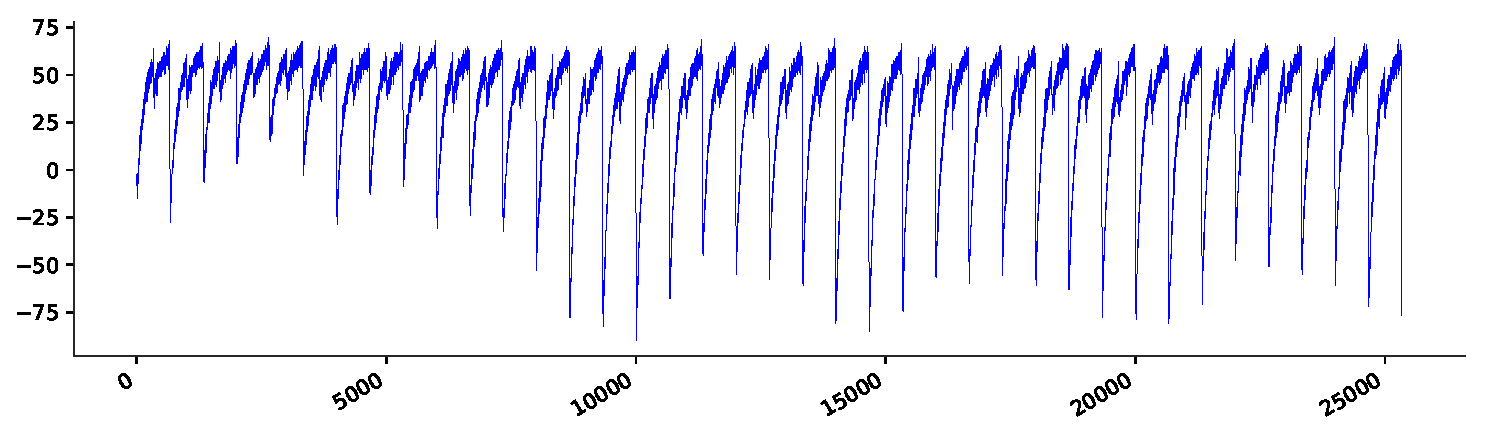
\includegraphics[scale=0.6]{traces/first_doubling/target_trace_dbl_oper_d64}
	\captionof{figure}{Target trace of the first doubling, which is produced using the value $d_{64} = 7$ with the base point and scalar as listed in \Cref{App sec: example template traces} in \Cref{Appendix}.}
	\label{fig: OTA first iteration target example}
\end{figure}
%
\begin{figure}
	\centering
	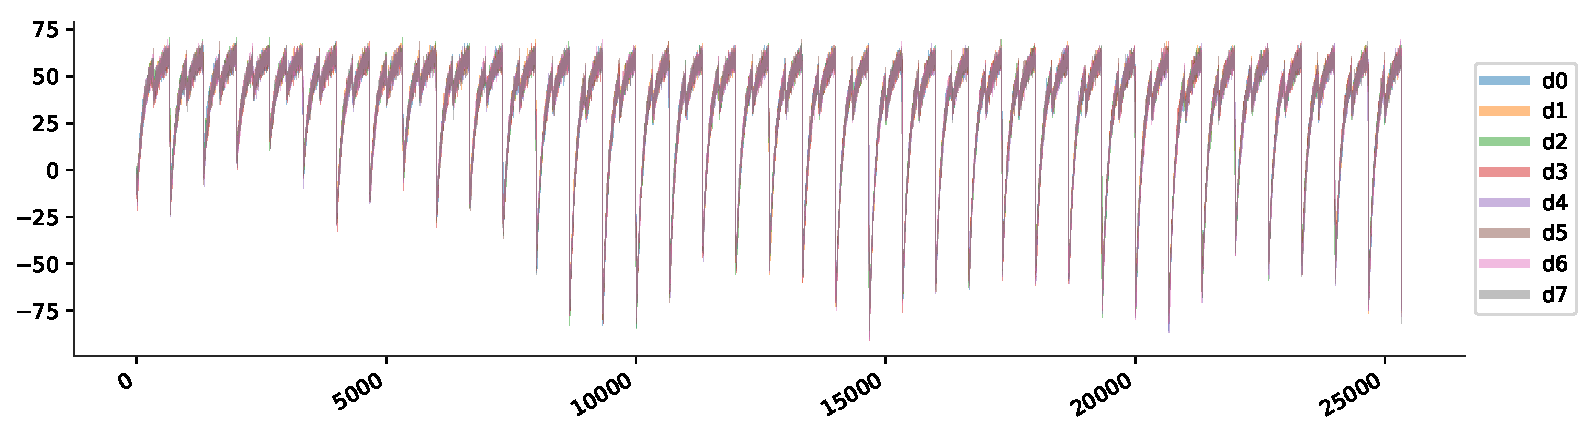
\includegraphics[scale=0.59]{traces/first_doubling/template_traces_overlap_d64}
	\captionof{figure}{An overlap of all the template traces shown in \Cref{App sec: example template traces}.}
	\label{fig: OTA first iteration template traces overlap}
\end{figure}
%
Without even looking at the correlation results, we can immediately see that the template traces are almost identical. 
After viewing the traces in Inspector SCA (a software product developed by Riscure), we can see that there are very small differences between these template traces.
The similarity among the template traces is also reflected in the correlation values obtained after correlating the templates with each other.
These correlation values are at least 99\%.

After correlating the template traces with the target trace using the Pearson correlation coefficient while attacking the first 5 digit-columns (i.e. the first 5 iterations of the OTA), we again observed that all of the correlation values were close to 99\%. 
Instead of only using the doubling operation, we also made use of the fact that we can use the addition operation to have two `operations of reference' instead of one.
Making use of this approach slightly decreased the correlation values.
However, the results were similar to the results observed when \emph{only} making use of the doubling operation.
We decided to research which part of the frequency of the target trace contained the expected leakage.
After applying FFT to the target trace, we found out that the interesting samples were in the higher frequencies of the trace.
This was verified by making use of a low-pass filter with a cut-off frequency of 81MHz.
If the interesting frequencies of a trace are filtered out, the traces will even look more similar, which will result in higher correlation values in the template-matching phase.
This is also exactly what we observed in the correlation values after we applied the aforementioned low-pass filter.
Therefore, we decided not to use this low-pass filter in the remaining experiments we conducted.

\subsection{Bandwidth filter comparison}
As the template-matching results are so close to each other, we decided to attack the first 5 digit-columns (i.e $d_{64}$ up to $d_{60}$) for the same target trace.
Each attack was performed 20 times with different bandwidth filters.
The reason for conducting this experiment is to get more insight in which settings of the oscilloscope are the most promising despite the high similarity among the template traces.
By performing the OTA 20 times using the same settings, we wanted to account for coincidences with respect to the ranking of the template that is expected to have the highest correlation value.
Results of the rankings for the correct template in attacking the first 5 digit-columns can be seen in \Cref{tbl: first 5 digit-columns bandwidth limit comparison}.
%
\begin{table}
	\centering
	%
	\subfloat[][Full.]{
		%	
		\begin{tabular}{*4c}
			\toprule
			& \bm{$\tilde{x}$} &  \bm{$\mu$} & \bm{$\sigma$}\\
			\midrule
				$d_{64}$ & 3.5 &  4.2 & 2.46 \\
				$d_{63}$ & 5.0 & 4.8  & 1.60  \\
				$d_{62}$ & 2.0 & 1.55 & 0.50 \\
				$d_{61}$ & 9.0 & 8.2  & 3.67 \\
				$d_{60}$ & 2.0 & 1.85 & 0.65 \\
			\bottomrule
		\end{tabular}
		%
		\label{tbl: first 5 digit-columns bandwidth full}
	}
	%	
	\vfill
	%
	\subfloat[][200MHz.]{
		%
		\begin{tabular}{*4c}
			\toprule
			& \bm{$\tilde{x}$} &  \bm{$\mu$} & \bm{$\sigma$}\\
			\midrule
			$d_{64}$ & 4.0 & 4.2 & 2.23\\
			$d_{63}$ & 5.5 & 4.55 & 2.18 \\
			$d_{62}$ & 1.5 & 1.5 & 0.50 \\
			$d_{61}$ & 5.5 & 6.4 & 3.83\\
			$d_{60}$ & 1.0 & 1.45 & 0.50\\
			\bottomrule
		\end{tabular}
		%
		\label{tbl: first 5 digit-columns bandwidth 200MHz}
	}
	\hspace{1cm}
	%
	\subfloat[][20MHz.]{
		%
		\begin{tabular}{*4c}
			\toprule
			& \bm{$\tilde{x}$} &  \bm{$\mu$} & \bm{$\sigma$}\\
			\midrule
			$d_{64}$ & 2.0 & 3.4 & 2.44\\
			$d_{63}$ & 4.0 & 3.85 & 1.65\\
			$d_{62}$ & 2.0 & 1.6 & 0.49\\
			$d_{61}$ & 11.5 & 10.5 & 3.61\\
			$d_{60}$ & 1.0 & 1.3 & 0.46\\
			\bottomrule
		\end{tabular}
		%
		\label{tbl: first 5 digit-columns bandwidth 20MHz}
	}
	\captionof{table}{The median ($\tilde{x}$), mean ($\mu$) and standard deviation ($\sigma$) of the rank of the correct template is shown after attacking the first 5 digit-columns. 
	These values were obtained after applying the OTA 20 times using the same target trace. 
	The number of times the expected template had the highest correlation value is 22, 28, and 31 for \protect\subref{tbl: first 5 digit-columns bandwidth full}, \protect\subref{tbl: first 5 digit-columns bandwidth 200MHz} and \protect\subref{tbl: first 5 digit-columns bandwidth 20MHz} respectively.}
	\label{tbl: first 5 digit-columns bandwidth limit comparison}
\end{table}
%
What is interesting to see is that the mean and median values for the rank of the correct template trace in attacking the digit-columns $d_{62}$ and $d_{60} $ is way lower than for the other digit-columns. 
This applies to each of the tables regardless the bandwidth filter applied.
It could be the case that the corresponding parts of the target trace are less noisy for these particular digit-columns, which causes the correct template to have the highest correlation value more often.
For the other digit-columns, it can be seen that both the mean and the standard deviation of the correct template are worse. 
Across most tables, the mean and standard deviations stay roughly the same. 
The mean value of the rank tends to go down for digit-column $d_{61}$ for a bandwidth limit of 200MHz \protect\subref{tbl: first 5 digit-columns bandwidth 200MHz} compared to the full bandwidth \subref{tbl: first 5 digit-columns bandwidth full}.

Based on the data shown in \Cref{tbl: first 5 digit-columns bandwidth limit comparison}, there seems to be no real difference between any of the bandwidth filters, which is probably due to the minimal differences between all of the correlation values. 
If we launch 20 OTA to attack the first 5 digit-columns, we have to make 100 guesses.
This applies to each of the tables shown in \Cref{tbl: first 5 digit-columns bandwidth limit comparison}.
In each of these guesses, we determine which template matches best with the target trace. 
If we compare this total number of guesses to the number of times we matched the correct templates for each of these tables, we get an indication on how bad the classification performance is: between 22-31\%. 
Despite the minimal differences between the number of templates matched correctly, we did however choose to settle with a bandwidth limit of 20MHz for the remaining experiments we conducted.
The reason for this choice is that this bandwidth limit resulted in the highest number of templates matched correctly.
We also note that this is the same bandwidth limit used in a side-channel attack (i.e. a correlation power analysis) on AES to test the performance of the SAKURA-G board once its development had finished \cite{guntur2014side}.
Besides experimenting with different values for the bandwidth limit (None, 20MHz or 200MHz), we also experimented with different sampling rates (from 500 MSa/s up to 20 GSa/s) and coupling values.
However, the correlation results for each possible configuration remained at least 99\% and gave no observable improvement over any of the other configurations we considered.

The high correlation values observed for each of the template traces are not in line with the results that were obtained in \cite{batina2014online}. 
In their experiments, it was observed that a correct template would give a correlation result that was much higher than a non-matching one (i.e. $\ge$97\% when correlating a matching template compared to 85\% for a non-matching template). 
These pattern-matching values would drop when multiple bits were attacked using a single acquisition (which was due to a stability problem with the power supply in their setup).
The previously mentioned results were however obtained on software devices.
These devices have different power properties compared to hardware devices such as FPGAs, which could make these result not directly applicable to our setup.

\subsection{Template averaging}
In \cite{dugardin2016dismantling} an OTA was launched against PolarSSL on an ARM architecture.
When they used a single (non-averaged) template trace to attack a key bit of the scalar, the correlation values observed for the correct templates were low.
They managed to increase the correlation results of the correct template by capturing a template trace multiple times and averaging these results.
By capturing the same template trace multiple times, one can somewhat account for the noise that is present in each acquired template trace.
The effectiveness of this approach depends on the number of additional template traces captured.
It was shown that the correct template had a correlation of 69\% when using a single template trace, while this number increased to 99.80\% when an average of 100 template traces was used.
In \Cref{tbl: first 5 digit-columns template averaging}, the results for applying this template-averaging technique to {\fourq} can be seen \Cref{tbl: first 5 digit-columns template averaging}.
%
\begin{table}
	\centering
	%
	\subfloat[][20 additional templates.]{
		\begin{tabular}{*4c}
			\toprule
			& \bm{$\tilde{x}$} &  \bm{$\mu$} & \bm{$\sigma$}\\
			\midrule
			$d_{64}$ & 3.0 & 3.3 & 1.79 \\
			$d_{63}$ & 5.0 & 5.3 & 1.62 \\
			$d_{62}$ & 1.0 & 1.4 & 0.49 \\
			$d_{61}$ & 6.5 & 6.2 & 3.06 \\
			$d_{60}$ & 2.0 & 1.6 & 0.49 \\
			\bottomrule
		\end{tabular}
	}
	%	
	\vfill
	%
	\subfloat[][50 additional templates.]{
		\begin{tabular}{*4c}
			\toprule
			& \bm{$\tilde{x}$} &  \bm{$\mu$} & \bm{$\sigma$}\\
			\midrule
			$d_{64}$ & 4.5 & 4.6 & 2.33 \\
			$d_{63}$ & 5.5 & 4.9 & 1.92 \\
			$d_{62}$ & 1.0 & 1.2 & 0.40 \\
			$d_{61}$ & 6.5 & 7.0 & 3.52 \\
			$d_{60}$ & 2.0 & 1.6 & 0.49 \\
			\bottomrule
		\end{tabular}
	}
	%	
	\hspace{1cm}
	%
	\subfloat[][100 additional templates.]{
		\begin{tabular}{*4c}
			\toprule
			& \bm{$\tilde{x}$} &  \bm{$\mu$} & \bm{$\sigma$}\\
			\midrule
			$d_{64}$ & 5.0 & 4.1 & 2.47\\
			$d_{63}$ & 4.0  & 3.6 & 1.47 \\
			$d_{62}$ & 1.0 & 1.4 & 0.49 \\
			$d_{61}$ & 6.0 & 6.3 & 3.63 \\
			$d_{60}$ & 2.0 & 1.6 & 0.49 \\
			\bottomrule
		\end{tabular}
	}	
	\captionof{table}{For each attack on the first 5 digit-columns, the median ($\tilde{x}$), mean ($\mu$) and the standard deviation ($\sigma$) of the rank of the correct template is shown when a bandwidth limit of 20MHz is used.
	The indicated number of additional traces (20, 50 or 100) are used to average the acquisition of a single template trace. Each OTA is performed 10 times.}
	\label{tbl: first 5 digit-columns template averaging}
\end{table}
%
As expected, the correlation values become higher once the number of additional template traces increases.
However, classification of the correct template is still far from optimal.
It is almost like throwing a dice to determine the rank of the correct template.
This is very clear if we look at the standard deviation of the rank of the expected template for both \Cref{tbl: first 5 digit-columns bandwidth limit comparison} and \Cref{tbl: first 5 digit-columns template averaging}. 
These results were obtained by making use of the same target trace (which would resemble a real-world scenario).
It could be the case that the attacked digit-columns at which the standard deviation is very high, the corresponding part of the target trace contains more noise than normal.
But due to the non-distinctiveness of the correct template trace, this reasoning remains speculation.
We also applied the averaging technique to the target trace itself (which does not represent a real-world scenario), but this did not yield any results that were more interesting than the usage of one (non-averaged) target trace.

\subsection{Preprocessing the traces}
As we can read in \Cref{subsec: template attacks preprocessing the traces} in \Cref{chp: Side Channel Attacks}, there are some preprocessing steps that we can take into account to improve template matching.
Also a method for selecting the most interesting points in a trace was applied (as described in \Cref{subsec: Making the attack more practical}).
These methods did however not yield improved results.
Besides that, we also made use of the built-in noise filter of the oscilloscope.
Digital oscilloscopes often have a sampling rate that is much higher than required.
This is called oversampling, and can be used to filter the digitized signal to either increase the effective resolution or to remove unwanted noise.
This method is called Enhanced Resolution (ERes).
With the oscilloscope used in our setup, oversampling can be used to increase the vertical resolution.
This is done by making use of moving-average filter \cite{waverunner6manual}.
Application of this particular filter did not gave any observable improvement, as the classification performance was almost identical as observed when applying the techniques discussed before.
Similarly, no improvements were observed with different sampling rates or coupling values of the channel used to capture the template/target trace.

% use Good article on impendance
% https://hackaday.com/2015/07/29/say-it-with-me-input-impedance/
